

%%%%%%%%%%%%%%%%%%%%%%%%%%%%%%%%%%%%%%%%%%%%%%%%%%%%%%%%%%%%%%%%

\subsubsection{End-wall coverage enhancement}

The eight calibration ports closer to the end-walls (four on each side) are not positioned on top of the \dword{tpc}, but instead located about \SI{40}{\cm} away from the \dword{fc} along the $z$ (beamline) direction. If positioned on top, \dword{fc} penetration would be quite complicated, having to come from the sides. Use of the periscope baseline design for the end-wall periscopes would severely limit the volume coverage, similar to the coverage limitation mentioned in Section~\ref{sec:sp-calib-sys-las-ion-des}.

We describe here an alternative design for the end-wall ports that would improve the laser beam coverage without requiring \dword{fc} penetration.
%or long horizontal tracks. 

The periscope is exactly the same as the baseline design but, at the top of the calibration port, is mounted on a flange that has an additional rotation degree of freedom. Figure~\ref{fig:laser_extrarotation} presents a preliminary drawing of the concept. The \SI{250}{\milli\m} diameter calibration port has on top of it the main rotary flange that, itself, has another smaller port off-centered by \SI{40}{\milli\m} with respect to the main one. On this smaller port, a secondary rotary flange is installed and it is this one that holds the laser periscope, including the optical feedthrough and the linear stage for mirror movement. When the main flange rotates, the periscope also moves along a circular (\SI{40}{\milli\m} diameter) trajectory. Consequently, within the cryostat, the relative position between the beam mirror and the \dword{fc} profiles changes as well, and so the shadowed regions also change, by parallax. Using different main rotary flange angles, it should be possible to locate the mirror in enough different positions in order to cover all the previously shadowed angles.

Calculations similar to the ones showed earlier show that, using only \num{3} different positions (separated by \ang{90}), a coverage of \SI{94}{\%} should be possible for \SI{30}{\cm} voxels and allowing all tracks directed at the \dword{apa}.

\begin{dunefigure}[CAD drawing of the double rotary flange for the end-wall laser calibration ports]{fig:laser_extrarotation}
{Exploded CAD drawing (preliminary) of the double rotary flange for the end-wall laser calibration ports. The calibration port is shown in brown at the bottom; the primary and secondary rotary flanges are shown in yellow,  with the (black) motors next to them. The optical feedthrough is shown in the center, in blue. On top, the mirror arrangement allows the laser beam to be aligned with the optical feedthrough no matter the angle of each of the rotary flanges.}
%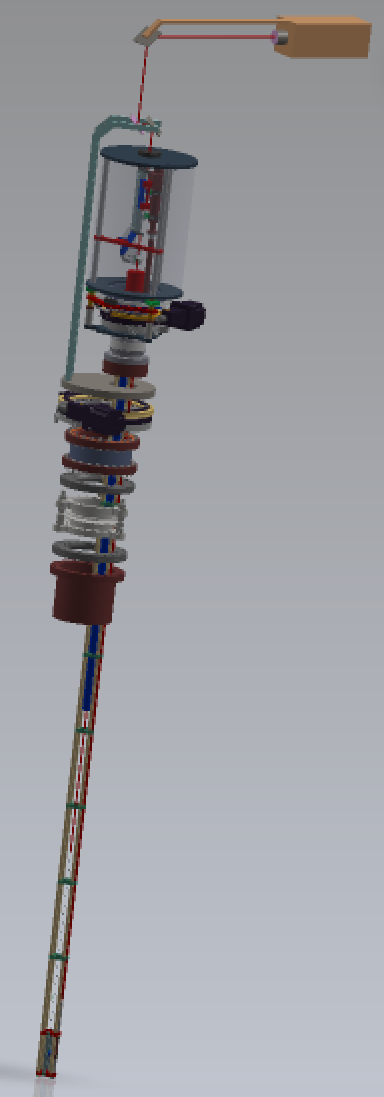
\includegraphics[width=0.24\linewidth]{laser_doublerotary1.png}
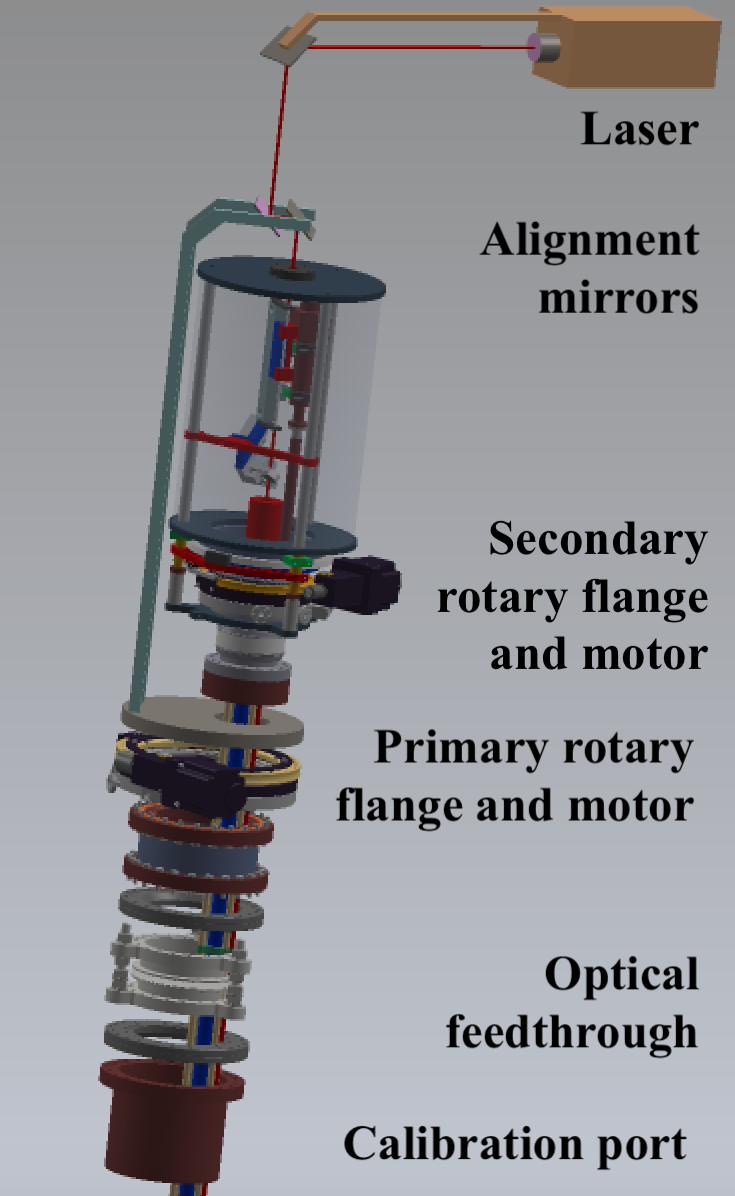
\includegraphics[width=0.4\linewidth]{calib-laser_doublerotary2_edit.png}
\end{dunefigure}
